\documentclass{article}
\usepackage{xeCJK}
\usepackage{amsmath}
\usepackage{listings}
\usepackage{xcolor}
\setlength{\parindent}{0pt}
\renewcommand{\baselinestretch}{1.0}
\lstset{
	frame=tb, % draw a frame at the top and bottom of the code block
	showstringspaces=false, % don't mark spaces in strings
	numbers=left, % display line numbers on the left
	commentstyle=\color{green}, % comment color
	keywordstyle=\color{blue}, % keyword color
	stringstyle=\color{red} % string color
}
\usepackage[a4paper,left=20mm,right=20mm,top=15mm,bottom=15mm]{geometry}  

\title{后缀自动机}
\author{MengChunlei}
\begin{document}
\maketitle
\begin{itemize}
	\item 定义
	\item 性质
	\item 算法
	\item 实现
\end{itemize}
\section{定义}
\subsection{前置定义}
\begin{itemize}
	\item 字符串$s$的长度定义为$|s|$
	\item 本文描述的字符串$s$的下标从0开始,即$s[0]$到$s[|s|-1]$.
	\item $s$中所包含的字符集为$\Sigma$,字符集大小为$|\Sigma |$
\end{itemize}
\subsection{SAM的定义}
\begin{itemize}
	\item 它是一棵树,节点表示状态,边为转移。每条边上是一个字符。从根节点到达某个节点的路径有很多条。一条路径上经过的所有边的字符连起来对应一个串。所以一个节点是一些串的集合。
	\item 根节点用$R$表示。
	\item 每个子串(包括后缀)对应树上一条唯一的路径。
	\item SAM是满足上述性质的节点数最少的树。
\end{itemize}
下面是一个$s=abcdcdd$的SAM. 右侧给出了每个节点代表的串的集合。 \par
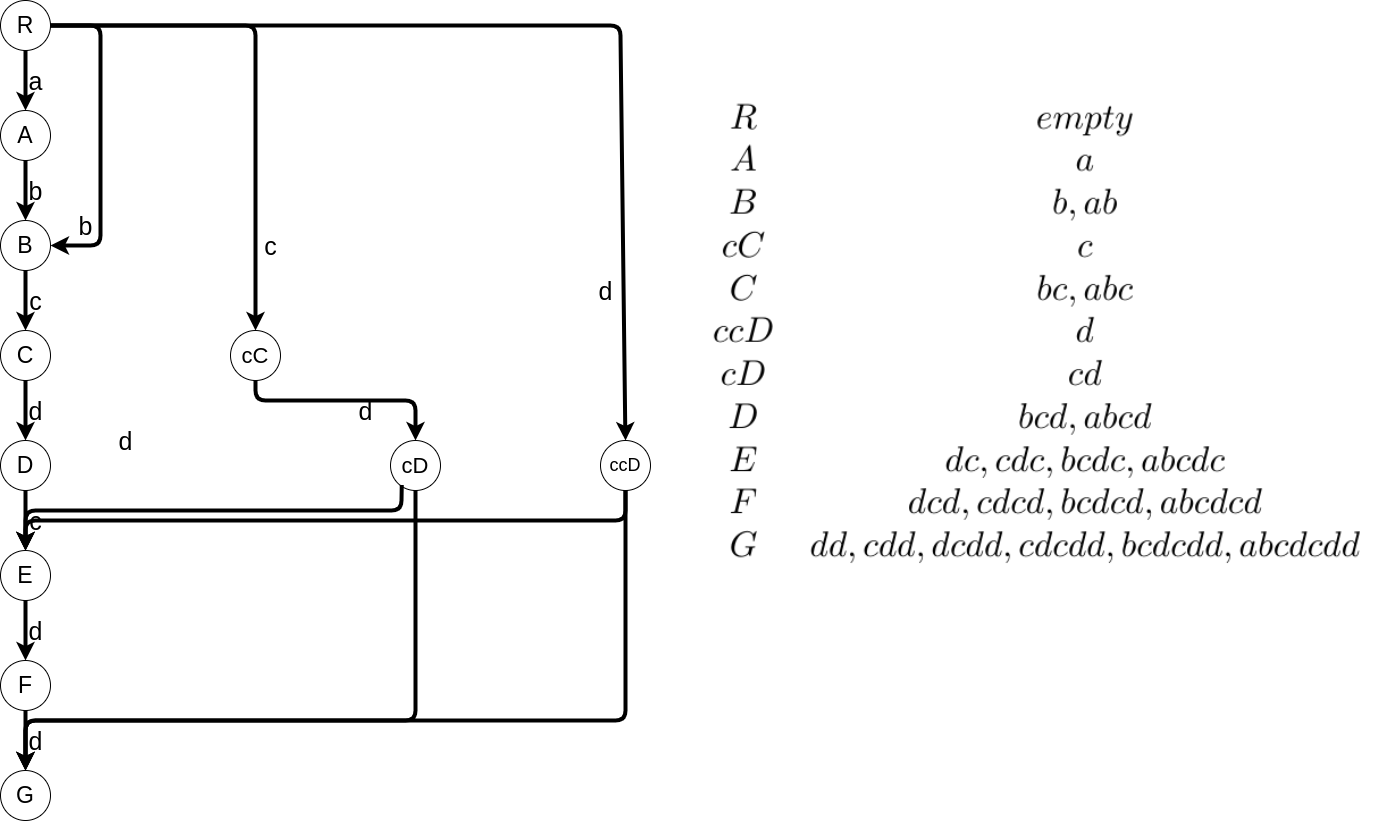
\includegraphics[scale=0.35]{pic1.png} \par
\subsection{endpos}
\begin{itemize}
	\item $endpos(t)$表示一个子串$t$出现的位置($t$的最后一个字符的位置)的集合,比如对于上面的例子,$endpos(cd)=\{2,4\}$
	\item 两个子串的$endpos$集合有可能相同,比如$endpos(bcd)=endpos(abcd)=\{3\}$
	\item $endpos$相同的串对应树上的同一个节点,也就是说,总的节点个数是不同的$endpos$的集合个数再加1(根节点)
\end{itemize}
$\begin{matrix} 
0 & 1 & 2 &3 & 4 & 5 &6\\ 
a & b & c &d & c & d &d\\ 
\end{matrix}$ \par
上面是字符串$s$的下标。下面最有一列是每个节点对应的$endpos$ \par
$\begin{matrix} 
R & empty & \{0,1,2,3,4,5,6\}\\ 
A & a & \{0\}\\
B & b,ab & \{1\}\\
cC & c & \{2,4\}\\
C & bc,abc & \{2\}\\
ccD & d & \{3,5,6\}\\
cD & cd & \{3,5\}\\
D & bcd,abcd & \{3\}\\
E & dc,cdc,bcdc,abcdc & \{4\}\\
F & dcd,cdcd,bcdcd,abcdcd & \{5\}\\
G & dd,cdd,dcdd,cdcdd,bcdcdd,abcdcdd & \{6\}\\
\end{matrix}$ \par

\section{性质}
\begin{itemize}
	\item 性质1: 两个子串$t_{1},t_{2}(|t_{1} \leq |t_{2}|)$的endpos集合相同,那么当且仅当$t_{1}$在$s$中的每次出现,都是以$t_{2}$的后缀出现
	\item 性质2: 两个子串$t_{1},t_{2}(|t_{1} \leq |t_{2}|)$,如果$t_{1}$是$t_{2}$的后缀,那么$endpos(t_{2}) \sqsubseteq endpos(t_{1})$,否则$endpos(t_{1})\sqcap endpos(t_{2})= \emptyset$
	\item 性质3: 对于一个等价类$Q=endpos$,设所有$endpos$为$Q$的字符串集合为$U$,比如上面的例子,对于$Q=\{3\}$来说,$U=\{bcd,abcd\}$。将$U$中的字符串按照长度递增排序,那么排在前面的字符串一定是后面的字符串的后缀。假设$U$中最长的串的长度为$maxl$,最短的为$minl$,那么$U$中的串的长度会覆盖区间$[minl,maxl]$.即每个长度都有一个串。
	\item 定义一种边后缀链接$link$:如果$u=link(v)$,那么表示从节点$v$沿着它的$link$边,会到达节点$u$.节点$v$对应一个等价类,假设这个等价类中串的长度区间为$[min_{v},max_{v}]$,同理假设节点$u$对应串的集合的长度区间为$[min_{u},max_{u}]$,那么满足$min_{v}=max_{u}+1$,并且$u$中所有的串都是$v$中所有串的后缀。即$link(v)$指向的节点是$v$中串最长后缀的另一个等价类。
	\item 性质4:后缀链接构成一棵以$R$为根的树。因为对于任意一个不是$R$的节点,沿着$link$边走所到达的节点对应的串集合中的最长的长度都会严格减少,所以一定能走到$R$.
	\item 性质5: link边形成的树跟$endpos$形成的树的节点一样.如下图所示。右侧为link边的树。
\end{itemize}
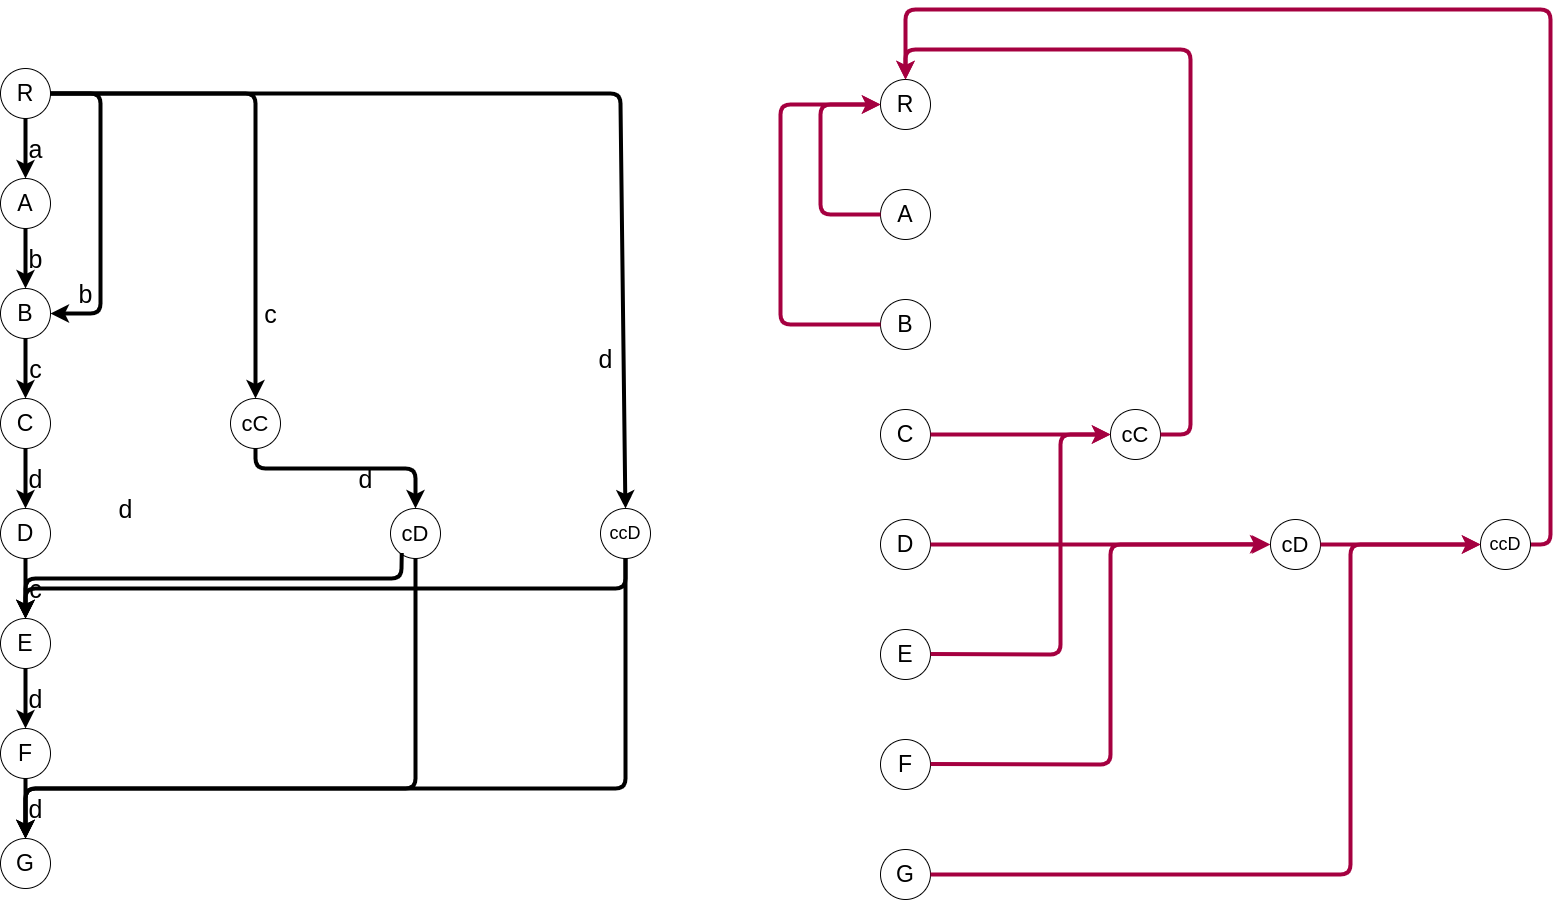
\includegraphics[scale=0.25]{pic2.png} \par

\section{算法}
下面以构建$s=abcdcdd$为例子。
\subsection{step0: R}
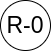
\includegraphics[scale=0.5]{step0.png} \par
初始时只有根节点。对应的$endpos$集合串的最长长度为0. R-0后面的0表示长度。\par

\subsection{step1: 插入$a$}
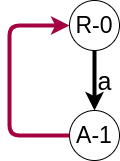
\includegraphics[scale=0.5]{step1.png} \par
首先构造一个新节点$A$,它的长度为1.先看转移边,由根节点通过一条$a$的转移边到达$A$. 再看$link$边,$A$节点对应的$endpos$集合为$\{0\}$,即串的集合为$\{a\}$,所以它的$link$边到达的串的长度为0(空串是串$a$的后缀),即$R$.\par

\subsection{step2: 插入$b$}
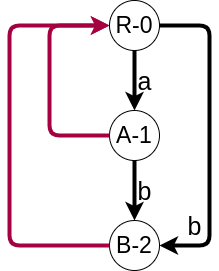
\includegraphics[scale=0.5]{step2.png} \par
首先构造一个新节点$B$,它的长度为2.先看转移边,由$A$节点通过一条$b$的转移边到达$B$.此时应该从$R=link(A)$也连一条$b$的转移边到$B$,因为$R$代表的串集合是$A$的真后缀。所以$B$对应的串集合为$\{b,ab\}$. 再看$link$边,$B$中所有串的真后缀为空串,它的$link$边到达的串的长度为0(空串是串$b$的后缀),即$R$.\par
\subsection{step3: 插入$c$}
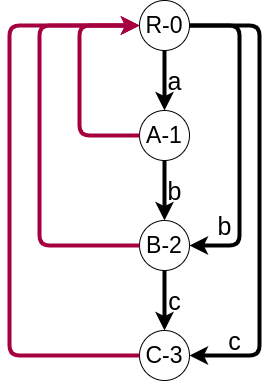
\includegraphics[scale=0.5]{step3.png} \par
插入$c$类似,节点$C$对应的串为$\{c,bc,abc\}$,对应的$endpos$为$\{2\}$ \par
\subsection{step4: 插入$d$}
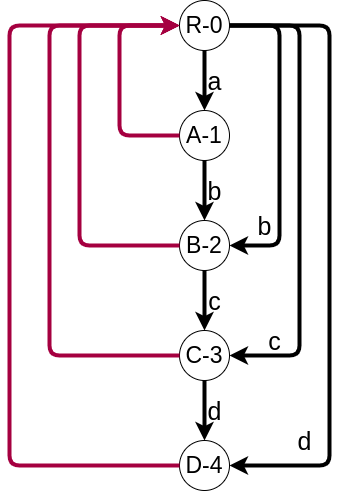
\includegraphics[scale=0.5]{step4.png} \par
插入$d$类似,节点$D$对应的串为$\{d,cd,bcd,abcd\}$,对应的$endpos$为$\{3\}$ \par

\subsection{step5: 插入$c$}
\subsubsection{step5-1: create E}
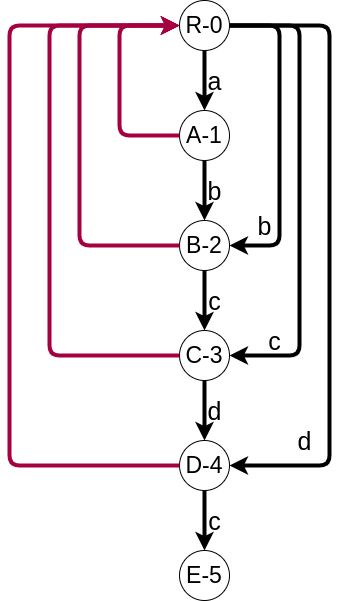
\includegraphics[scale=0.5]{step51.png} \par
首先新建一个节点$E$,设置长度为5.并从$D$连一条$c$的边到$E$.这时,$E$代表的串为$\{dc,cdc,bcdc,abcdc\}$,即$D$表示的串后面加上字符$c$. 这时候理论上还要从$R=link(D)$连一条$c$的边到$E$(表示$R$对应的串加上$c$).但是这时候$R$已经有一条$c$的边了,是到节点$C$。这时候的解决思路是把$E$和$C$的公共部分抽取出来。 \par
\subsubsection{step5-2: clone C}
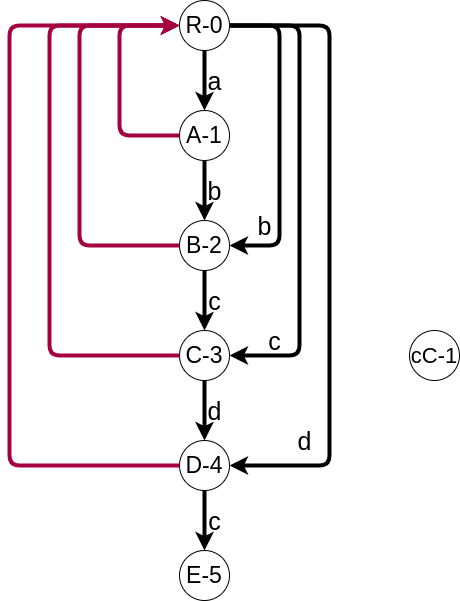
\includegraphics[scale=0.5]{step52.png} \par
这时候新建一个节点$cC$(clone C).它表示的串是$C=\{c,bc,abc\}$和$E=\{c,dc,cdc,bcdc,abcdc\}$的公共部分,即$C \sqcap E = \{c\}$,所以$cC$的长度为1.这时候$C$应该只表示$C=\{bc,abc\}$.

\subsubsection{step5-3: rebuild connection}
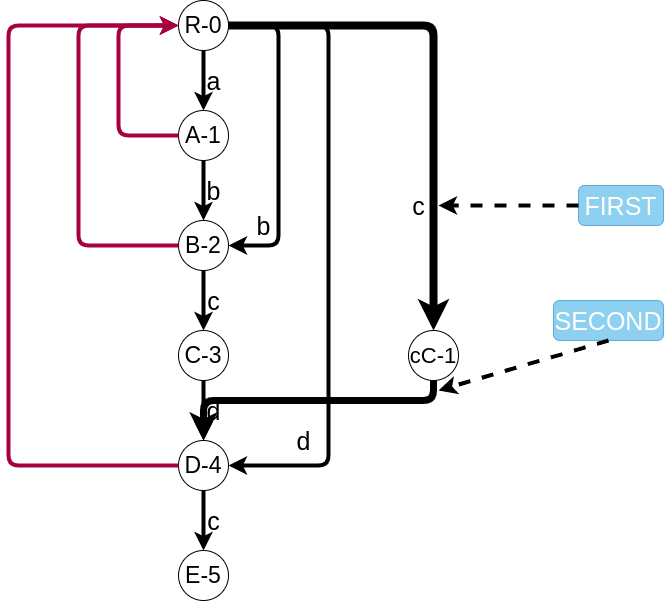
\includegraphics[scale=0.5]{step53.png} \par
\begin{itemize}
	\item 第一个修改,将$R$出发的字符为$c$的边从$C$改为指向$cC$,因为这时候$cC$表示串$\{c\}$
	\item 第二个修改,所有从$C$出发的边(不包括link边)都要copy一份到$cC$上,即$cC$也要有一条到$D$的字符为$d$的边,否则$D$将丢失串$cd$.
\end{itemize}
\subsubsection{step5-4: update link}
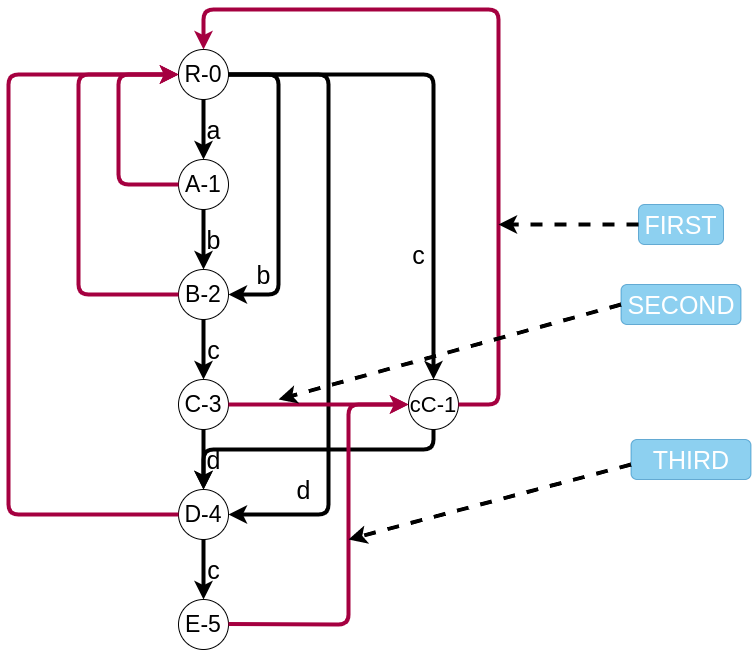
\includegraphics[scale=0.5]{step54.png} \par
\begin{itemize}
	\item $cC$的$link$指向$R$:$\{c\}$的后缀为空串
	\item $C$的$link$指向$cC$,即$\{bc,abc\}$的最长后缀为$\{c\}$
	\item $E$的$link$指向$cC$,即$\{dc,cdc,bcdc,abcdc\}$的最长后缀为$\{c\}$
\end{itemize}

\subsection{step6: 插入$d$}
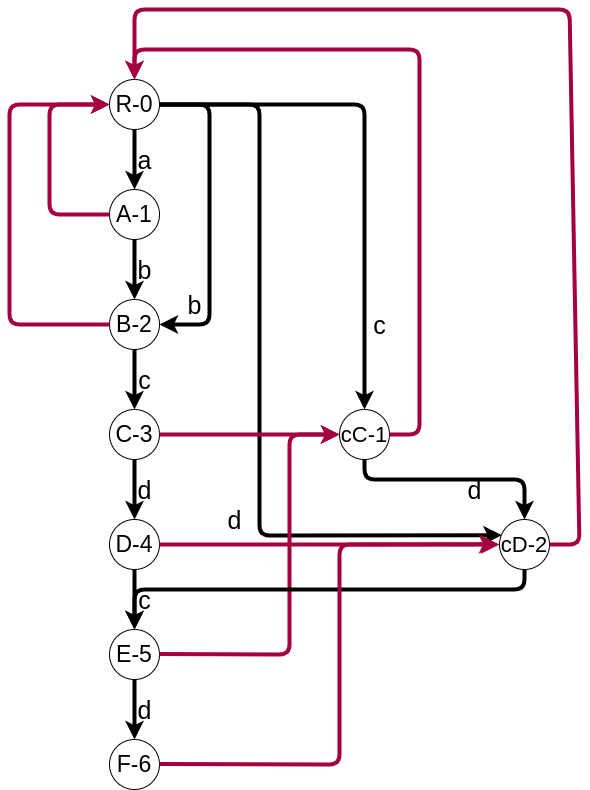
\includegraphics[scale=0.35]{step6.png} \par

\subsection{step7: 插入$d$}
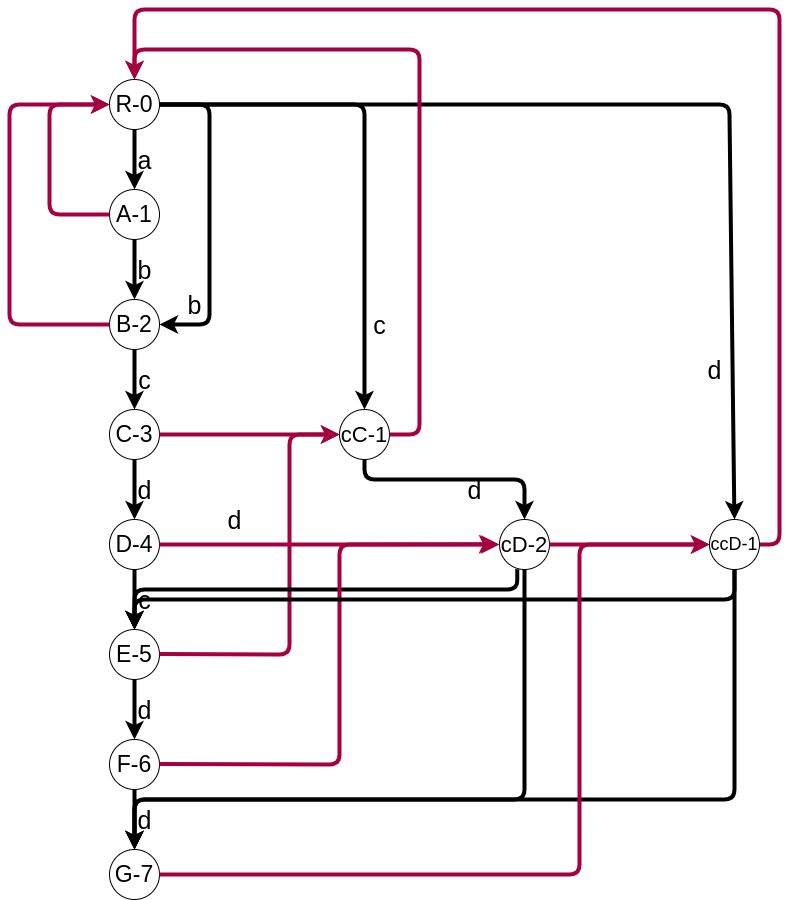
\includegraphics[scale=0.5]{step7.png} \par

\section{实现}
\subsection{数据结构定义}
\begin{lstlisting}[language=C++, caption={Definition}]
class SAM {
public:
  SAM(int size) : pools(size * 2), use_index(1), last_index(0) {
    pools[0].length = 0;  /*The R is index 0*/
    pools[0].link = -1;
  }
private:
  struct Node {
    int length;
    int link;
    std::unordered_map<int, int> next;
  };
  std::vector<Node> pools;
  int use_index;
  int last_index;
};
\end{lstlisting}

\subsection{插入字符}
\begin{lstlisting}[language=C++, caption={Insert}]
void SAM::Add(int c) {
  int curr_index = use_index++;
  Node &curr = pools[curr_index];
  Node &last = pools[last_index];
  curr.length = last.length + 1;
  int p = last_index;
  while (p != -1 && 0 == pools[p].next.count(c)) {
    pools[p].next[c] = curr_index;
    p = pools[p].link;
  }
  if (p == -1) {
    curr.link = 0;
  } else {
    int q = pools[p].next[c];
    if (pools[p].length + 1 == pools[q].length) {
      curr.link = q;
    } else {
      int clone_index = use_index++;
      Node &clone = pools[clone_index];
      clone.length = pools[p].length + 1;
      clone.next = pools[q].next;
      clone.link = pools[q].link;
      for (; p != -1 && pools[p].next[c] == q; p = pools[p].link) {
        pools[p].next[c] = clone_index;
      }
      pools[q].link = curr.link = clone_index;
    }
  }
  last_index = curr_index;
}
\end{lstlisting}

\end{document}
